\documentclass{article}
\usepackage[UTF8, heading = false, scheme = plain]{ctex}

\usepackage{geometry}
\geometry{b5paper,left=2cm,right=2cm,top=2cm,bottom=2cm}

\usepackage{color}
\usepackage{amsfonts}
\usepackage{amsmath}

\linespread{1.5}

\usepackage[colorlinks,
            linkcolor=red,
            anchorcolor=blue,
            citecolor=green
            ]{hyperref}
\usepackage{graphicx}
\usepackage{listings}
\usepackage{fontspec}
\newfontfamily\monaco{Monaco}
\definecolor{dkgreen}{rgb}{0,0.6,0}
\definecolor{gray}{rgb}{0.5,0.5,0.5}
\definecolor{mauve}{rgb}{0.58,0,0.82}
\lstset{ %
  basicstyle=\footnotesize\monaco,       % the size of the fonts that are used for the code
  numbers=left,                   % where to put the line-numbers
  numberstyle=\footnotesize\monaco\color{gray},  % the style that is used for the line-numbers
  numbersep=5pt
  stepnumber=1,                   % the step between two line-numbers. If it's 1, each line
                                  % will be numbered
  numbersep=5pt,                  % how far the line-numbers are from the code
  backgroundcolor=\color{white},      % choose the background color. You must add \usepackage{color}
  showspaces=false,               % show spaces adding particular underscores
  showstringspaces=false,         % underline spaces within strings
  showtabs=false,                 % show tabs within strings adding particular underscores
  frame=single,                   % adds a frame around the code
  rulecolor=\color{black},        % if not set, the frame-color may be changed on line-breaks within not-black text (e.g. commens (green here))
  tabsize=4,                      % sets default tabsize to 2 spaces
  captionpos=t,                   % sets the caption-position to bottom
  breaklines=true,                % sets automatic line breaking
  breakatwhitespace=false,        % sets if automatic breaks should only happen at whitespace
  title=\lstname,                   % show the filename of files included with \lstinputlisting;
                                  % also try caption instead of title
  keywordstyle=\color{blue},          % keyword style
  commentstyle=\color{dkgreen},       % comment style
  stringstyle=\color{mauve},         % string literal style
  escapeinside={\%*}{*)},            % if you want to add LaTeX within your code
  morekeywords={*,...}               % if you want to add more keywords to the set
}

\usepackage{amssymb} 

\setlength{\parindent}{2em}

\renewcommand{\G}{\mathbb{G}}
\newcommand{\Z}{\mathbb{Z}}
\newcommand{\Q}{\mathbb{Q}}
\newcommand{\F}{\mathbb{F}}

\newcommand{\Sbox}{\textsf{Sbox}}
\newcommand{\code}[1]{\lstinline!#1!}

%%%%%%%处理下划线:_%%%%%%%%%
\usepackage{underscore}
%%%%%%%处理下划线:_%%%%%%%%%

\setlength{\parindent}{2.1em}

%%%设置页眉和页码格式
\usepackage{fancyhdr}
\newcommand{\makeheadrule}{%
\rule[0.85\baselineskip]{\headwidth}{0.5pt}\vskip-.8\baselineskip}%1.5 0.4->0.5
\makeatletter
\renewcommand{\headrule}{%
{\if@fancyplain\let\headrulewidth\plainheadrulewidth\fi
\makeheadrule}}
\makeatother
\pagestyle{fancy}
\fancyhf{}
\fancyhead[r]{\textit{Crypto In Action}}
\fancyfoot[C]{--{~\thepage~}--}
%%%设置页眉和页码格式结束

\usepackage{color}
\newcommand{\red}{\textcolor{red}}
\newcommand{\blue}{\textcolor{blue}}


\begin{document}

\title{基于secp256k1的自同态映射加速ECDSA验签}
\author{longcpp \\ \small{longcpp9@gmail.com}}

\maketitle

由于Bitcoin的采纳,基于椭圆曲线secp256k1的ECDSA签名机制在区块链领域得到广泛应用.
Bitcoin最开始采用的是OpenSSL中实现的基于secp256k1的ECDSA签名机制,
然而OpenSSL中没有针对曲线secp256k1进行针对性优化,也就导致OpenSSL中基于secp256k1曲线的ECDSA效率很差.
值得注意的是, OpenSSL项目中对基于secp256r1曲线的ECDSA进行了深度优化.
 
%OpenSSL中的两种ECDSA的实现速度测试在Listing~\ref{openssl-bench}~中给出.
% \lstinputlisting[firstline=9, lastline=72, caption=\texttt{openssl_ecdsa_benchmark},label=openssl-bench]{./openssl-bench.cpp}


编译链接OpenSSL 1.1版本,在Intel(R) Core(TM) i7-6700HQ CPU上的执行结果显示
OpenSSL提供的基于secp256k1的ECDSA的执行速度大约为2000  sign/s和2300 verify/s,
而基于secp256r1的ECDSA的执行速度大约为33000 sign/s和12000 veriy/s.
可以说OpenSSL中基于secp256k1曲线的ECDSA实现比基于secp256r1曲线的ECDSA实现慢了一个数量级.
安全性方面,根据~\cite{ecdsa-side-channel}中结论显示OpenSSL 1.1中的基于secp256k1的ECDSA实现是不安全的.

OpenSSL实现的速度安全问题以及OpenSSL版本变动可能引入的不一致问题(参考DER编码和BIP 66)
不能满足区块链场景下对速度,安全以及稳定性的要求, Bitcoin核心开发者在libsep256k1项目中重新实现了
基于secp256k1的ECDSA, 针对曲线secp256k1做了深度优化并同时保证了常量实现.
采纳基于secp256k1的ECDSA机制的区块链项目目前都默认采用libsec256k1中的实现.

libsep256k1项目中采用了大量技巧以提升签名验签的执行效率,
这里我们仅关注利用secp256k1的自同态(Endomorphism)特性提升验签效率.
开始讨论技术之前,首先感受下自同态特性的利用在libsecp256k1项目中带来的速度提升,
注意为了利用自同态特性加速验签过程,需要在~\code{./configure}~时候指定~\code{--enable-endomorphism}~选项.
另外libsecp256k1还提供了选项~\code{--with-bignum=gmp|no},可以利用GMP中实现进一步提升速度.
为了利用libsec256k1自带的速度测试用例,也同时需要指定~\code{--enable-benchmark}.
Listing~\ref{lst-openssl-libsecp256k1-bench}~中列出了
指定不同的编译选项(是否使用GMP库以及是否开启自同态选项)时,
利用libsecp256k1自带的性能测试工具得到的测试数据.
%编译时不指定~\code{--enable-endomorphism}~选项,利用libsecp256k1自带的测试工具执行结果如下:


\begin{lstlisting}[caption=\texttt{ECDSA with secp256k1 benchmark, OpenSSL vs libsecp256k1 }, label=lst-openssl-libsecp256k1-bench]
# no gmp, no endomorphism, 12330 veiry/s
secp256k1 git:(master) ./configure --enable-benchmark --with-bignum=no
secp256k1 git:(master) ./bench_verify
ecdsa_verify: min 80.0us / avg 81.1us / max 82.5us
ecdsa_verify_openssl: min 498us / avg 510us / max 522us

# with gmp, no endomorphism, 14320verify/s
secp256k1 git:(master) ./configure --enable-benchmark --with-bignum=gmp
secp256k1 git:(master) ./bench_verify
ecdsa_verify: min 68.6us / avg 69.8us / max 70.7us
ecdsa_verify_openssl: min 498us / avg 510us / max 522us

# no gmp, with endomorphism, ~15950 verify/s
secp256k1 git:(master) ./configure --enable-benchmark --with-bignum=no --enable-endomorphism
secp256k1 git:(master) ./bench_verify
ecdsa_verify: min 61.6us / avg 62.7us / max 66.5us
ecdsa_verify_openssl: min 498us / avg 510us / max 522us

# with gmp, with endomorphism, ~19800 verify/s
secp256k1 git:(master) ./configure --enable-benchmark --with-bignum=gmp --enable-endomorphism
secp256k1 git:(master) ./bench_verify
ecdsa_verify: min 49.9us / avg 50.5us / max 51.4us
ecdsa_verify_openssl: min 498us / avg 510us / max 522us
\end{lstlisting}

%\begin{lstlisting}[caption=\texttt{libsecp256k1 benchmark without --enable-endomorphism}]
%$  secp256k1 git:(master) ./bench_sign
%ecdsa_sign: min 45.6us / avg 46.1us / max 48.3us
%$  secp256k1 git:(master) ./bench_verify 
%ecdsa_verify: min 65.4us / avg 66.5us / max 68.6us
%ecdsa_verify_openssl: min 471us / avg 474us / max 476us
%\end{lstlisting}

%编译时指定\code{--enable-endomorphism}选项,利用libsecp256k1自带的效率测试工具执行结果如下:

%\begin{lstlisting}[caption=\texttt{libsecp256k1 benchmark with --enable-endomorphism}]
%$  secp256k1 git:(master) ./bench_sign  
%vecdsa_sign: min 45.5us / avg 46.1us / max 48.2us
%$  secp256k1 git:(master) ./bench_verify 
%ecdsa_verify: min 47.0us / avg 47.6us / max 49.6us
%ecdsa_verify_openssl: min 470us / avg 476us / max 490us
%\end{lstlisting}

%可以看到,是否指定选项~\code{--enable-endomorphism}~对于libsecp256k1的ECDSA签名速度没有影响,
%每次签名耗时大约为46 us, 也即大约为22000 sign/s. 
可以看到同时指定选项~\code{--enable-endomorphism}~和~\code{--with-bignum=gmp}~验签时,
验签速度最快,大约50.5us即可完成一次验签操作,相比不使用这两个选项时的81.1us,有了大约37\%的速度提升.
仅使用~\code{--with-bignum=gmp}~选项时,大约有14\%的速度提升,
而仅使用~\code{--enable-endomorphism}~时,大约有22\%的速度提升.
%从平均66.5 us提高至平均47.6 us,也即从15000 verify/s提高至21000 verify/s, 大约有40\%的速度提升.
值得注意的是, libsecp256k1的速度测试工具中同时测试了OpenSSL中基于secp256k1的ECDSA的运行速度,
每次验签操作耗大约耗时510us,大约为2000 verify/s.
libsecp256k1指定不同的编译选项时的速度,以及OpenSSL中基于secp256k1和secp256r1的ECDSA速度对比在
在Table~\ref{tbl-ecdsa-bench}~中给出, 本文接下来关注自同态特性的原理.

\begin{table}[h]
\centering
\caption{ECDSA速度对比}\label{tbl-ecdsa-bench}
\begin{tabular}{|c|c|c|c|c|c|}
\hline
\small
         & OpenSSL & OpenSSL & libsecp256k1  & libsecp256k1 \\
         & secp256r1 & secp256k1 & secp256k1        & secp256k1 \\
         &                 &                 &   no end, no gmp & end, gmp \\\hline
 sign/s  & 31000  & 1900 & 20800 & 20800 \\\hline
 verify/s & 11600 & 2000 & 12300 & 19800 \\\hline
\end{tabular}
\end{table}

早在2011年, Bitcoin开发者Hal Finney就在bitcointalk论坛上指出
可以利用secp256k1的自同态特性加速ECDSA的验签操作~\cite{halfinney}, 并给出了原理示例代码.
浏览libsecp256k1的代码实现可知, libsecp256k1中的实现是以Hal Finney的示例为基础的,
而Hal Finney的原理示例则基于~\cite{guidetoecc}~中Section 3.5节中的内容,
而Section 3.5节中的内容来自论文~\cite{glv01}.

假设$E$是定义在域(Field) $K$上的椭圆曲线,用$E$表示该椭圆曲线上的所有的点的集合,
则$E$上的自同态(Endomorphism)映射是满足
$$\phi(\mathcal{O}) = \mathcal{O}, \phi(P) = (g(P), h(P)), \forall P \in E$$
的映射$\phi: E \rightarrow E$, 其中$g$和$h$是系数位于$K$的有理函数(Rational Function).
如果$\phi_1$和$\phi_2$上自同态映射,则定义两者的和$\phi_1+\phi_2$为$(\phi_1+\phi_2)(P) = \phi_1(P) + \phi_2(P)$.
定义两者的乘积$\phi_1\phi_2$为$(\phi_1\phi_2)(P)=\phi_1(\phi_2(P))$.在这样的加法和乘法的定义下,
$E$上的所有的自同态映射构成一个环(Ring),称为域$K$上$E$的自同态环(Endomorphism Ring of $E$ over $K$).
值得注意的是,自同态映射$\phi$同时也是一个群同态映射(Group Homorphism),满足
$$\phi(P_1 + P_2) = \phi(P_1) + \phi(P_2), \forall P_1, P_2 \in E.$$

假设$p$是一个满足$p\equiv 1 \mod 3$的大素数, $E$则是定义在$\F_p$上的椭圆曲线$E: y^2 = x^3 + b$,
用$\beta$表示$\F_p$上一个阶(Order)为3的元素, 则有$E$上的自同态映射
$$\phi(x,y) \rightarrow (\beta x, y), \phi(\mathcal{O}) = \mathcal{O}.$$
将$(\beta x, y)$带入$E$的方程有$y^2 = (\beta x)^3 + b = \beta^3x^3 + b$可以看到$\phi$确实是$E$到自身的映射.
由于$order(\beta)=3$ ($\beta^3 \equiv 1 \mod p$),则$y^2 = (\beta x)^3 + b = \beta^3x^3 + b  = x^3 + b$.
自同态映射$\phi: E \rightarrow E$的特征多项式(Characteristic Polynomial)为$X^2 + X + 1$.
一个自同态映射$\phi$的特征多项式是$\Z[X]$中满足
$f(\phi)=0$(也即$f(\phi)(P)=\mathcal{O}, \forall P\in E$)的次数最小的首一多项式$f(X)$.
接下来验证自同态映射$\phi$确实满足$f(\phi)(P)=\mathcal{O}, \forall P\in E$, 也即
$$(\phi^2+\phi+1)(P) = \mathcal{O}, \forall P \in E.$$
假设$P=(x,y)$, 则根据自同态环的定义有
$$(\phi^2+\phi+1)(P) = \phi^2(P) + \phi(P) +1(P) = (\beta^2 x, y) + (\beta x, y) + (x,y)$$
根据~\cite{Blahut14}中给出的点加运算示例,参见Figure~\ref{fig-ecpoint-add},有
 $$(\beta^2 x, y) + (\beta x, y) + (x,y) = (-\beta^2 x -\beta x, -y) + (x,y).$$
 由于$\beta^3 \equiv 1 \mod p$,就有$\beta^2+\beta+1=0$,则
$$ (-\beta^2 x -\beta x, -y) + (x,y) = (-(\beta^2+\beta) x, -y) = (x,-y) + (x,y) = \mathcal{O}.$$
 
\begin{figure}
\centering
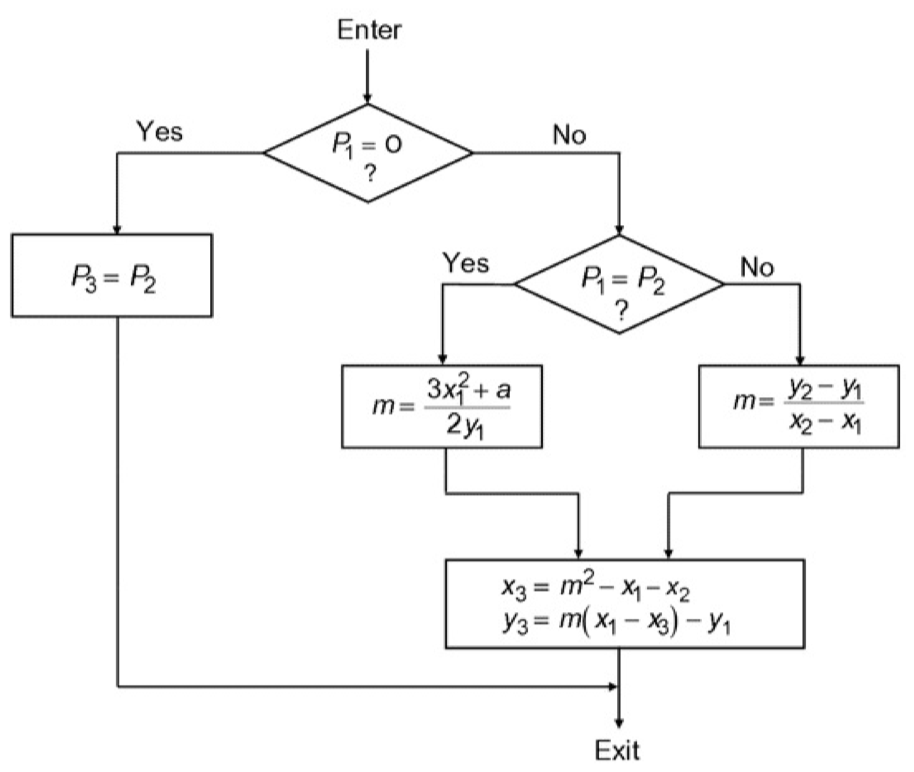
\includegraphics[width=.7\textwidth]{ec-point-addition.png}
\caption{$y^2=x^3+b$的点加运算$(x_3,y_3)=P_3=P_1+P_2=(x_1,y_1) + (x_2,y_2)$}\label{fig-ecpoint-add}
\end{figure}

用$\#E(\F_p)$表示集合$E(\F_p)$中点的个数,其中$p \equiv 1 \mod 3$是素数,
用$n$表示$\#E(\F_p)$的最大素因子并且$n^2 \nmid \#E(\F_p)$,
则点群$E(\F_p)$仅包含一个阶为$n$的子群(Subgroup),记这个子群的基点(Base Point)为$G\in E(\F_p)$, 
记这个子群为$\G = \langle G \rangle$. 
假设$\phi(G)\neq \mathcal{O}$,则前述的映射$\phi$相当于$\G$上的一个点倍乘映射:
$$
\phi(G) = \lambda G, \lambda^2+\lambda+1\equiv 0 \mod n.
$$

考虑定义在有限域$\F_p$上的曲线secp256k1: $y^2 = x^3 + 7$,其中
\small
$$p = 0xfffffffffffffffffffffffffffffffffffffffffffffffffffffffefffffc2f.$$
\normalsize
$\#E(\F_p) = h \cdot n$,其中$h = 1$为余因子(Cofactor), $n$为$E(\F_p)$的最大素子群的阶:
\small
$$ n = 0xfffffffffffffffffffffffffffffffebaaedce6af48a03bbfd25e8cd0364141.$$
\normalsize
子群 $\langle G \rangle$的基点$G$的坐标为:
$$G_x = 0x79be667ef9dcbbac55a06295ce870b07029bfcdb2dce28d959f2815b16f81798$$
$$G_y = 0x483ada7726a3c4655da4fbfc0e1108a8fd17b448a68554199c47d08ffb10d4b8$$
注意到secp256k1的参数$p\equiv 1 \mod 3, n | \#E(\F_p), n^2 \nmid \#E(\F_p)$,则存在自同态映射$\phi$:
$$
\phi(P) = \phi(x, y) = (\beta x, y) = \lambda P, \beta^3 \equiv 1 \mod p, \lambda^2 + \lambda + 1 \equiv 0 \mod n, \forall P \in \G.
$$
由于
$$\lambda P = (\beta x, y) \rightarrow \lambda^2 P = (\beta^2 x, y) \rightarrow \lambda^3 P = (\beta^3 x, y) = (x, y),$$
也即$\lambda^3 \equiv 1 \mod n$ ($\lambda^2+\lambda + 1 \equiv 0 \mod n$).
根据费马小定理(Fermat's Little Theorem),可以按照Listing~\ref{lst-betalamb}~计算$\beta, \lambda$的值.

\begin{lstlisting}[language=python, caption=\texttt{generate $\beta$ and $\lambda$ for endomorphism of secp256k1}, label=lst-betalamb]
sage: p = 0xfffffffffffffffffffffffffffffffffffffffffffffffffffffffefffffc2f
sage: n = 0xfffffffffffffffffffffffffffffffebaaedce6af48a03bbfd25e8cd0364141
sage: fp = GF(p)
sage: fn = GF(n)
sage: beta = fp(2)^((fp.characteristic()-1)/3)
sage: lamb = fn(3)^((fn.characteristic()-1)/3)
sage: hex(int(beta))
'0x7ae96a2b657c07106e64479eac3434e99cf0497512f58995c1396c28719501eeL'
sage: hex(int(lamb))
'0x5363ad4cc05c30e0a5261c028812645a122e22ea20816678df02967c1b23bd72L'
\end{lstlisting}

根据$\beta, \lambda$的具体取值以及secp256k1的参数,可以用具体数值验证前述理论,
e.g. $(\phi^2+\phi + 1)(P) = \mathcal{O}$ 以及 $\lambda P = (\beta x, y)$,参见Listing~\ref{lst-verifyphi}.

\begin{lstlisting}[language=python, caption=\texttt{verify endomorphism $\phi$ with $\beta, \lambda$ for secp256k1}, label=lst-verifyphi]
sage: secp256k1 = EllipticCurve(fp, [0,7])
sage: P = secp256k1.random_point()
sage: beta_P = int(lamb) * P
sage: beta2_P = int(lamb * lamb) * P
sage: secp256k1.is_on_curve(P.xy()[0], P.xy()[1])
True
sage: secp256k1.is_on_curve(beta_P.xy()[0], beta_P.xy()[1])
True
sage: secp256k1.is_on_curve(beta2_P.xy()[0], beta2_P.xy()[1])
True
sage: P + beta_P + beta2_P
(0 : 1 : 0)
sage: P
(41377969691400010933106372906063172361899533199914561951528196380352494104025 : 
98022602531930804648533646821930292808872917654793309549219646753654843391634 : 1)
sage: beta_P
(61065808270983873313809816182282167124533426070191311711991257449293116444501 : 
98022602531930804648533646821930292808872917654793309549219646753654843391634 : 1)
sage: beta2_P
(13348311274932311176654795920342568366837025395534690375938130178263224123137 : 
98022602531930804648533646821930292808872917654793309549219646753654843391634 : 1)
sage: beta * P.xy()[0]
61065808270983873313809816182282167124533426070191311711991257449293116444501
sage: beta * beta * P.xy()[0]
13348311274932311176654795920342568366837025395534690375938130178263224123137
\end{lstlisting}

secp256k1上的自同态映射可以用来加速点的倍乘,能够加速ECDSA的验签过程,参见~\cite{stallings}中给出的Figure~\ref{fig-ecdsa}.
注意签名过程中涉及到只有固定点$G$的倍乘运算$kG$,点的倍乘运算利用预计算方法可以高效计算,无需利用自同态映射
\footnote{这句需要进一步验证, 固定点计算应用自同态映射是否会更快?直觉上不会}.
验证过程中,需要计算$es^{-1}G+rs^{-1}Q$,其中的$rs^{-1}Q$部分可以利用自同态映射进行加速,其中$(r,s)$为签名值,
$e$为待签名消息的哈希值.接下来讨论如何利用自同态$\phi$加速非固定点的倍乘运算,从而加速ECDSA的验签效率.

\begin{figure}[h]
\centering
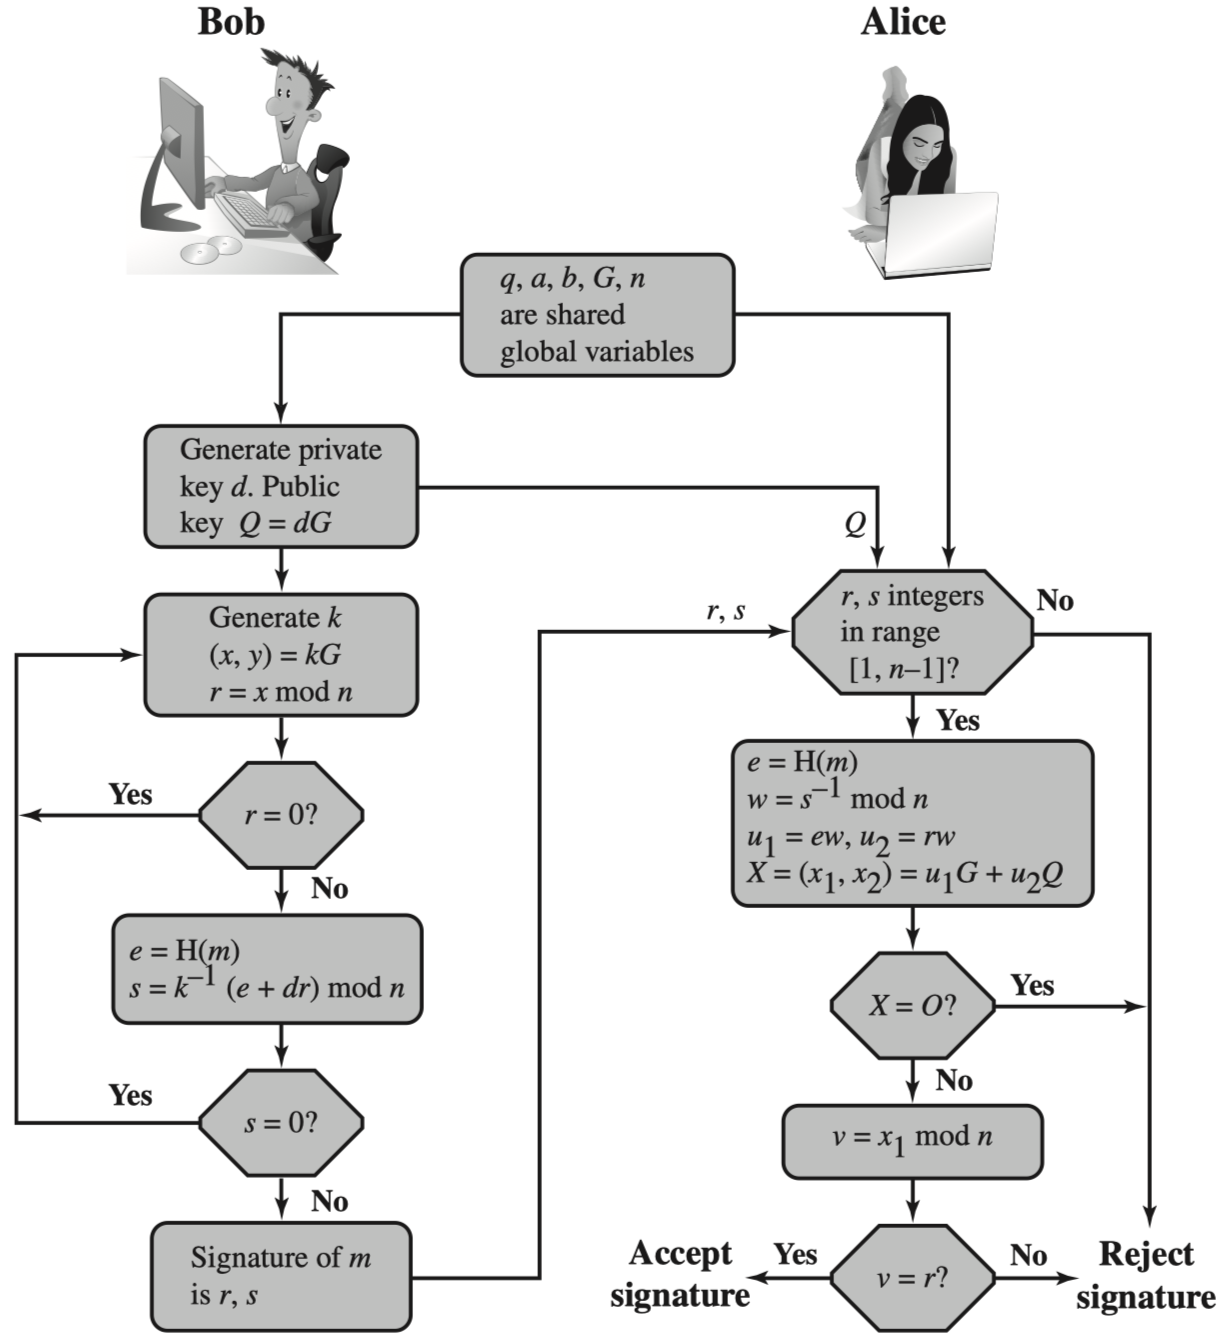
\includegraphics[width=.8\textwidth]{ecdsa.png}
\caption{ECDSA签名验签}\label{fig-ecdsa}
\end{figure}

记待计算的点倍乘运算为$kP$,将标量$k$表示为$k=k_1+k_2\lambda \mod n$,其中$k_1, k_2$的比特长度大约是$k$的一半,则有
$$kP = k_1P + k_2\lambda P = k_1P + k_2\phi(P) = k_1 P + k_2 Q, Q = \phi(P)$$
其中$Q=\phi(P)$仅需要一次域中的乘法运算($(x_Q, y_Q) = (\beta x_P, y_P)$),
而$k_1 P + k_2 Q$的计算可以利用多点并行乘法(Simultaneous Multiple Point Multiplication)完成.

标量$k$的分解$k \equiv k_1+k_2\lambda \mod n$在~\cite{glv01}中有讨论,完整的算法参见~\cite{guidetoecc}~中的Algorithm 3.74.
分解$k$的算法,输入为$n, \lambda, k\in [1, n-1]$,输出结果为$(k_1, k_2) \in \Z \times \Z$满足
$k \equiv k_1 + k_2 \lambda \mod n$,并且$(k_1, k_2)$的欧几里得范数(Euclidean Norm)较小.
考虑定义为$(i,j) \rightarrow i + j\lambda$的同态映射$f: \Z\times\Z \rightarrow \Z_n$,
我们希望找到的是向量$\mathbf{k}=(k_1, k_2)\in \Z\times\Z$并且满足$f(\mathbf{k})= k$.
注意$\mathbf{k} = (k, 0)$满足上述要求,但是这种值对我们加速点倍乘的初衷没有任何帮助,
我们需要的是具有小的欧几里得范数的向量$\mathbf{k}$.

~\cite{glv01}中给出的求解思路是首先找到两个线性独立(Linearly Independent)的向量$\mathbf{v_1}, \mathbf{v_2} \in \Z \times \Z$
并且有$f(\mathbf{v_1}) = f(\mathbf{v_2}) = 0$. 然后计算由$\mathbf{v_1}, \mathbf{v_2}$
生成的接近$(k,0)$的向量$\mathbf{v} = \beta_1\mathbf{v_1} + \beta_2\mathbf{v_2}$,
则$\mathbf{k} = (k,0) - \mathbf{v}$是满足$f(\mathbf{k}) = f((k,0)) - f(\mathbf{v}) = k$的短向量.

可以利用扩展的欧几里得算法(Extended Eculidean Algorithm)寻找向量$\mathbf{v_1}$和$\mathbf{v_2}$.
将扩展的欧几里得算法应用到$n$和$\lambda$, 则计算过程中会产生一系列的等式:
\begin{equation}
\label{eq-eea}
s_i n + t_i \lambda = r_i, i = 0, 1, 2, ....
\end{equation}
其中$s_0 = 1, t_0 = 0, r_0 = n, s_1 =0, t_1 = 1, r_1 = \lambda$并且有$r_i \ge 0$.
则有如下性质:
\begin{enumerate}
\item $r_i > r_{i+1} \ge 0 \text{ for all } i \ge 0$
\item $|s_i| < |s_{i+1}| \text{ for all } i \ge 1$
\item $|t_i| < |t_{i+1}| \text{ for all } i \ge 0$
\item $r_{i-1}|t_i| + r_i|t_{i-1}| = n \text{ for all } i \ge 1$
\end{enumerate}
第2点和第3点可以从扩展的欧几里得算法计算$s_i$和$t_i$的过程中看出.
\begin{equation}\nonumber
s_i = \left\{
\begin{array}{ll}
1 & \text{ if } i = 0 \\
0 & \text{ if } i = 1, \\
s_{i-2} - q_{i-1}s_{i-1} & \text{ if } i \ge 2 
\end{array}
\right. 
t_i = \left\{
\begin{array}{ll}
0 & \text{ if } i = 0 \\
1 & \text{ if } i = 1 \\
t_{i-2} - q_{i-1}t_{i-1} & \text{ if } i \ge 2 
\end{array}
\right.
\end{equation}
可知$s_2 = 1$, $s_3$是负数,则$s_4 = s_2 - q_3s_3$为正数,可以看到随着$i$的增大,
$s_i$的正负号交替变换,从而有$|s_i| < |s_{i+1}| \text{ for all } i \ge 1$.
同理可证明$|t_i| < |t_{i+1}| \text{ for all } i \ge 0$.
第4点性质可以通过归纳法证明. $i = 1$时, $r_0|t_1| + r_1|t_0| = n \cdot 1 + \lambda \cdot 0 = n$.
假设$r_{i-1}|t_i| + r_i|t_{i-1}| = n$成立,考察$r_{i}|t_{i+1}| + r_{i+1}|t_{i}|$:
\begin{equation}\nonumber
\begin{split}
r_{i}|t_{i+1}| + r_{i+1}|t_{i}| = & r_{i}|t_{i-1} - q_{i}t_{i}| + (r_{i-1}-q_{i}r_{i})|t_{i}| \\
= & r_i|t_{i-1}| + r_iq_i|t_i| + r_{i-1}|t_i| - q_ir_i|t_i|\\
= & r_i|t_{i-1}|+ r_{i-1}|t_i| = n.
\end{split}
\end{equation}
记$m$为满足 $r_m \ge \sqrt{n}$的最大的$m$,根据上述第4条性质就有$r_m|t_{m+1}| + r_{m+1}|t_m| = n$, 可推断$|t_{m+1}|<\sqrt{n}$.
根据Equaiton (\ref{eq-eea})有
$$s_{m+1}n + t_{m+1}\lambda = r_{m+1} \rightarrow r_{m+1} - t_{m+1} \lambda = s_{m+1} n \equiv 0 \mod n.$$
取$(a_1, b_1) = \mathbf{v_1}  = (r_{m+1}, - t_{m+1})$,就能满足$f(\mathbf{v_1}) = 0$.
由于$|t_{m+1}|<\sqrt{n}$以及$|r_{m+1}| < \sqrt{n}$, 则$\mathbf{v_1}$的欧几里得范数$||\mathbf{v_1}|| <\sqrt{2n}$.
取$(a_2, b_2) = \mathbf{v_2}$为$(r_{m}, - t_{m})$和$(r_{m+2}, - t_{m+2})$中欧几里得范数较小的那个,则根据Equaiton (\ref{eq-eea})有$f(\mathbf{v_2}) = 0$.直观上感觉,$\mathbf{v_2}$在所有满足条件的向量中也具有较小的欧几里得范数.
可以注意到$\mathbf{v_1}$和$\mathbf{v_2}$是相互独立的,不失一般性假设$\mathbf{v_2}=(r_m,-t_m)$,则有
$$
\dfrac{r_{m+1}}{r_m} = \dfrac{-t_{m+1}}{-t_m} = \dfrac{t_{m+1}}{t_m},
$$
由于$\frac{r_{m+1}}{r_m} < 1$以及$|\frac{t_{m+1}}{t_m}| > 1$,产生矛盾.

有了$\mathbf{v_1}$和$\mathbf{v_2}$之后,构建接近$(k,0)$的向量$\mathbf{v} = \beta_1\mathbf{v_1} + \beta_2\mathbf{v_2}$,
由于在$\Z\times\Z$结构上并不一定存在$\beta_1, \beta_2 \in \Z$
能够使$\mathbf{v} = \beta_1\mathbf{v_1} + \beta_2\mathbf{v_2}$成立.
所以在$\Q\times\Q$结构上考虑, e.g. $\beta_1, \beta_2 \in \Q$,
求得$\beta_1, \beta_2$之后, 在$\Z$中选取距离$\beta_1, \beta_2$最近的整数$c_1, c_2$,
则$\mathbf{v} = c_1\mathbf{v_1} + c_2\mathbf{v_2}$, 则期望构建的向量 
$$\mathbf{k} = (k,0) - \mathbf{v} = (k, 0) - c_1\mathbf{v_1} + c_2\mathbf{v_2},$$
其中, $k_1 =  k - c_1a_1 - c_2a_2, \ k_2 = \ -c_1b_1-c_2b_2$.

\begin{figure}[h]
\centering
\caption{\cite{guidetoecc}~中的Algorithm 3.74: 分解$k$}\label{fig-splitk}
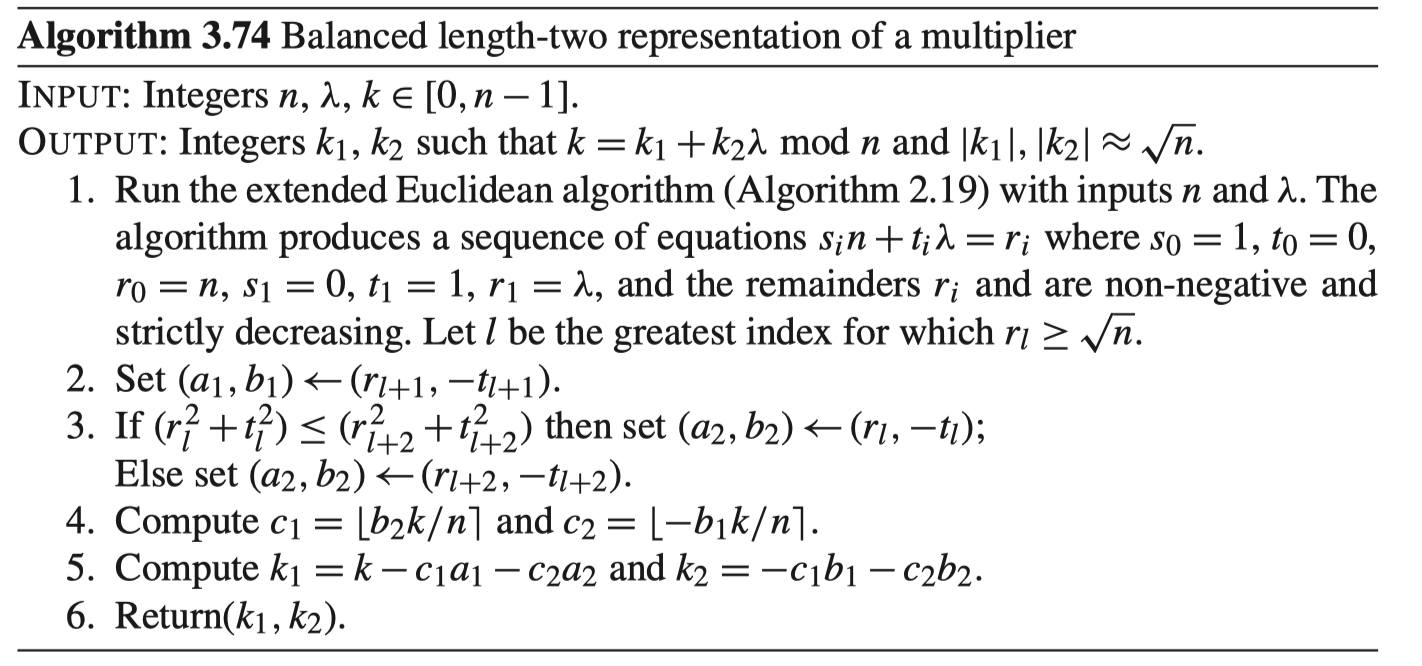
\includegraphics[width=\textwidth]{split-k.png}
\end{figure}


接下来考察如何计算$\beta_1, \beta_2$.由于$(k, 0) = \beta_1(a_1,b_1) + \beta_2(a_2, b_2)$, 就有
\begin{equation}\nonumber
\begin{split}
\beta_1a_1 + \beta_2a_2 =& \  k\\
\beta_1b_1 + \beta_2b_2 =& \ 0
\end{split}
\end{equation}
解方程组可以得到
$$\beta_1 = \dfrac{b_2k}{a_1b_2 - a_2b_1}, \ \beta_2 = \dfrac{-b_1k}{a_1b_2-a_2b_1}.$$
由于$(a_1, b_1) = (r_{m+1}, - t_{m+1})$,并且不失一般性有$(a_2, b_2) = (r_{m}, - t_{m})$, 
根据前述第4点性质,以及$t_i$序列中相邻两个值的符号相反,则有
$$|a_1b_2-a_2b_1| = |-r_{m+1}t_{m}+ t_{m+1}r_{m}| = n,$$
进而可以得到
$$\beta_1 = b_2k / n, \ \beta_2 = -b_1k/n, \ c_1 = \lfloor \beta_1 \rceil, \  c_2 = \lfloor \beta_2 \rceil.$$
根据上述讨论,可以理解~\cite{guidetoecc}~中的Algorithm 3.74,参见Figure~\ref{fig-splitk}.

Listing~\ref{lst-splitk}~中展示了用Sage实现的Figure~\ref{fig-splitk}~中$k$分解算法,为了验证正确性,也同时输出了
$a_1, b_1, a_2, b_2, c_1, c_2$的值.与~\cite{halfinney}对比发现输出的$a_1, b_1, a_2, b_2, c_1, c_2$值与Finney给出的一致.

\lstinputlisting[caption=\texttt{split_k with $\lambda$ for secp256k1},label=lst-splitk]{./split-k.sage}

为了进一步验证$k$分解的有效性, Listing~\ref{lst-splitkverify}~中对随机选取的$k\in_R[1,n-1]$,用$\lambda$进行了分解,
可以发现~\code{split_k}~返回的$k_1, k_2$,满足$k_1 + k_2\lambda\equiv k\mod n$.
\begin{lstlisting}[language=python, caption=\texttt{verify multiplier split  with $\lambda$ for secp256k1}, label=lst-splitkverify]
sage: load("split-k.sage")
sage: k = int(fn.random_element())
sage: k1, k2 = split_k(n, int(lamb), k)
k 0x572d5beb0549d2ddcb1ff17bc516568c7f2a4d776e9c15d86e42ae55396f34f5L
a1, b1 0x3086d221a7d46bcde86c90e49284eb15L -0xe4437ed6010e88286f547fa90abfe4c3L
a2, b2 0x114ca50f7a8e2f3f657c1108d9d44cfd8L 0x3086d221a7d46bcde86c90e49284eb15L
c1, c2 0x10866a88d9692d0cb6a3e3188351f370L 0x4dbb61ed92bcc5654a28486a8793676aL
k1, k2 0x4cfc491368f8e9bb17180d76c4587555L 0x6bb2c62e9346d862c0edd4a2cf1e649eL
sage: (k1 + k2 * int(lamb)) % n
39431360339721158570738739562322678290810515502148100028669271620139548095733
sage: k
39431360339721158570738739562322678290810515502148100028669271620139548095733L
\end{lstlisting}

基于$a_1, b_1, a_2, b_2, c_1, c_2$的值Finney在~\cite{halfinney}中给出了基于OpenSSL的PoC代码.
由于OpenSSL版本变动导致的接口变化问题,Finney的代码需要稍微修改才能在OpenSSL 1.1版本下编译通过.
调整之后的代码参见Listing~\ref{lst-endpoc},编译之后的执行的结果显示利用自同态特性有大约16\%左右的速度提升.

\lstinputlisting[firstline=67, lastline=155, firstnumber=67, caption=\texttt{PoC of speeding up ECDSA verification with endomorphism},label=lst-endpoc]{./secp256k1-endomorphism.c}

libsecp256k1中仅使用~\code{--enable-endomorphism}~选项时22\%的速度提升整合了更多的优化技巧,
例如通过预计算避免在分解$k$的时候执行除法运算等,留作以后分析.

\begin{thebibliography}{99}

\bibitem{ecdsa-side-channel}
Genkin, Daniel, Lev Pachmanov, Itamar Pipman, Eran Tromer, and Yuval Yarom. "ECDSA key extraction from mobile devices via nonintrusive physical side channels." In Proceedings of the 2016 ACM SIGSAC Conference on Computer and Communications Security, pp. 1626-1638. ACM, 2016.

\bibitem{halfinney}
Hal Finney. bitcointalk - Speeding up signature verification. 2011.
\url{https://bitcointalk.org/index.php?topic=3238.0}

\bibitem{guidetoecc}
Hankerson, Darrel, Alfred J. Menezes, and Scott Vanstone. "Guide to elliptic curve cryptography." Computing Reviews 46, no. 1 (2005): 13.

\bibitem{Blahut14}
Blahut, Richard E. Cryptography and secure communication. Cambridge University Press, 2014.

\bibitem{stallings}
Stallings, William. Cryptography and network security: principles and practice. Upper Saddle River: Pearson, 2017.

\bibitem{glv01}
Gallant, Robert P., Robert J. Lambert, and Scott A. Vanstone. "Faster point multiplication on elliptic curves with efficient endomorphisms." In Annual International Cryptology Conference, pp. 190-200. Springer, Berlin, Heidelberg, 2001.

\end{thebibliography}

\end{document}